
%%%%%%%%%%%%%%%%%%%%%%% file typeinst.tex %%%%%%%%%%%%%%%%%%%%%%%%%
%
% This is the LaTeX source for the instructions to authors using
% the LaTeX document class 'llncs.cls' for contributions to
% the Lecture Notes in Computer Sciences series.
% http://www.springer.com/lncs       Springer Heidelberg 2006/05/04
%
% It may be used as a template for your own input - copy it
% to a new file with a new name and use it as the basis
% for your article.
%
% NB: the document class 'llncs' has its own and detailed documentation, see
% ftp://ftp.springer.de/data/pubftp/pub/tex/latex/llncs/latex2e/llncsdoc.pdf
%
%%%%%%%%%%%%%%%%%%%%%%%%%%%%%%%%%%%%%%%%%%%%%%%%%%%%%%%%%%%%%%%%%%%


\documentclass[runningheads,a4paper]{llncs}

\usepackage{amssymb,amsmath}
\setcounter{tocdepth}{3}
\usepackage{graphicx}
\DeclareMathOperator*{\argmin}{arg\,min}
\usepackage{subfigure, caption}

\usepackage{url}
%\urldef{\mailsa}\path{a.churchill,ssgd,c.t.fernando}@qmul.ac.uk
\newcommand{\keywords}[1]{\par\addvspace\baselineskip
\noindent\keywordname\enspace\ignorespaces#1}

\begin{document}

\mainmatter  % start of an individual contribution

% first the title is needed
\title{An Estimation of Distribution-like Algorithm based on a Denoising Autoencoder}

% a short form should be given in case it is too long for the running head
\titlerunning{An EDA-like Algorithm based on a Denoising Autoencoder}

% the name(s) of the author(s) follow(s) next
%
% NB: Chinese authors should write their first names(s) in front of
% their surnames. This ensures that the names appear correctly in
% the running heads and the author index.
%
\author{Alex%
%
\and Sid\and Chrisantha}
%
\authorrunning{Alex, Sid and Chrisantha}
% (feature abused for this document to repeat the title also on left hand pages)

% the affiliations are given next; don't give your e-mail address
% unless you accept that it will be published
\institute{School of Electronic Engineering and Computer Science\\Queen Mary, University of London\\
{\{a.churchill,ssgd,c.t.fernando\}}@qmul.ac.uk}

%
% NB: a more complex sample for affiliations and the mapping to the
% corresponding authors can be found in the file "llncs.dem"
% (search for the string "\mainmatter" where a contribution starts).
% "llncs.dem" accompanies the document class "llncs.cls".
%

\toctitle{Lecture Notes in Computer Science}
\tocauthor{Authors' Instructions}
\maketitle


\begin{abstract}
In this paper we present a novel neural-based optimisation algorithm. The algorithm follows the traditional generate-update methodology of Estimation of Distribution algorithms, using a denoising autoencoder to learn the structure of promising solutions within its hidden layer, with the output neurons defining a probability distribution that is sampled from to produce new solutions. The algorithm is shown to outperform a canonical Genetic Algorithm on several combinatorial problems, including the multidimensional 0/1 knapsack problem, MAXSAT and the Hierarchical If and Only If. Analysis shows that the neural network is able to learn interesting structural features of the search space, while the sampling method employed supports continued exploration, enabling optimal solutions to be found on NP-hard problems.
\end{abstract}


\section{Introduction}

Estimation of Distribution Algorithms (EDAs) are a growing area in Evolutionary Computation, which attempt to statistically model sections of a search space in order to uncover underlying structure and guide search towards optimal solutions in an efficient manner \cite{pelikan2006scalable}. At the heart of any EDA lies a model-building algorithm. Examples include Bayesian Networks \cite{hboa}, Markov Networks \cite{ref} and K-Means clustering \cite{ref}. In this paper we introduce a novel neural-based method for modelling, a denoising autoencoder. An autoencoder is a feed forward neural network, consisting of at least one hidden layer, which is trained to reproduce its inputs from its outputs. Over the course of training the hidden layer learns a compressed representation of the data, which has been used for reconstructing missing data \cite{ref} and dimensionality reduction \cite{ref} in Machine Learning applications. The algorithm introduced in this paper trains a single autoencoder with promising solutions from a population, learning structural features of the search space in the hidden layer representation. This differs from traditional EDAs such as PBIL \cite{ref } or ECGA \cite{ref} as an explicit statistical model is not produced. However, the learnt structure can be leveraged to produce new solutions by inputting an existing or randomly generated solution into the network and sampling from the output neurons using a Bernoulli distribution. Results presented in Section 5 show that the autoencoder method is able to outperform a canonical Genetic Algorithm (GA) across a range of combinatorial and hierarchical problems.

\section{Background}

EDAs (also known as Probabilistic-Model-Building Genetic Algorithms) are population based optimisers, that typically replace genetic operators with a statistical model. The rationale behind the model building and related linkage learning approach is that dependencies between variables can be captured and preserved, which can be easily lost in standard Evolutionary Search, and new solutions generated around promising structures. Early work on EDAs concentrated on methods that explicitly modelled the probabilities of features occurring independently in a population of genotypes. These include the compact Genetic Algorithm \cite{cha}, PBIL \cite{phil} and Univariate Marginal Probability methods\cite{uvmp}. Improved success was found by modelling multivariate dependencies using clustering algorithms (ECGA) \cite{ecga}, Bayesian Networks \cite{hboa}, Markov Networks \cite{mccall} and tree structures \cite{ltga}, among others.

The use of the autoencoder model in this paper is motivated by its potential to learn high-dimensional non-linear dependencies in data, while maintaining a low computational cost in terms of training time. Recently there has been interest in neural-based methods in an EDA context for multi-objective optimisation. A Growing Neural Gas (GNG) was used as a model in \cite{moneda}, employing a competitive Hebbian learning rule to cluster data without having to pre specify the number of groups. A shallow Restricted Boltzmann Machine (RBM) was used to model high dimensional data in \cite{singapore}, beating the state-of-the-art on several multi-objective continuous benchmark problems. An autoencoder is another neural-based method for the unsupervised learning of features and has hitherto not been applied to combinatorial or continuous optimisation.

A second motivation for this approach is to investigate methods in which Evolutionary Algorithms can be implemented using neural structures. The {\em{Neural Replicator Hypothesis}} \cite{ref} proposes that evolutionary processes could operate in the brain at ontogenetic timescales. In \cite{fernando2010neuronal}, a (1+1)-ES is implemented in a network of spiking neurons. Adding Hebbian learning enabled linkages to be found between features, and the 128-bit HIFF problem to be solved.

\section{Sid's Shit}
EDAs attempt to probabilistically model the population of best solutions at each generation and produce new solutions by sampling from this model. Therefore an EDA algorithm consists of two main components, model building/estimation and sampling. 

EDAs vary in the complexity of the models that are employed for modelling distributions. More complex models are better at capturing structure from the training data, however they are often hard to train and can lead to significantly longer computational times. However, difficult problems may require the use of such complex models, without which convergence is impossible. 

The data generating distribution for high dimensional data is often very complex and is modelled better with complex probabilistic models. This improvement in modelling capacity helps improve performance of an EDA \cite{pelikan2002survey}. There are several EDAs that use complex probabilistic models to model the distribution of individuals at every generation [RBM,hBOA,etc etc]. 

In this work, we propose a model that uses a denoising autoencoder for learning to model the structure of the best solutions and to generate new solutions at each iteration.
A standard autoencoder is a model that learns the structure or distribution of the training data by means of a layer of latent or hidden variables. An autoencoder is comprised of an encoder and decoder network. Training is performed by minimising the error in reconstructing the input given the hidden representation.  The encoder network is a non-linear generalisation of PCA \cite{hinton2006reducing}. The autoencoder learns interactions between the input attributes and maps it to the hidden layer via a non-linear transformation, making it a powerful model for learning structure. 

In our algorithm we use a denoising autoencoder (dA) which is a variant of the standard autoencoder \cite{vincent2008extracting}. The denoising autoencoder tries to recreate the input from `corrupted' or `noisy' versions of the input. Autoencoders are trained along with strong regularisation in order to impose an information bottleneck on the model. If this is not done carefully, it would be very easy for the autoencoder to learn the identity transformation which would not be very useful. Adding the denoising criterion to the model forces the model to learn more robust representations which are invariant when the input is partially corrupted. Although denoising was introduced in order to encourage the learning of more robust representations, in our system we employ the denoising criterion to widen the basins of attraction around the best individuals in every generation. During training, we train the autoencoder on the most promising solutions, and by increasing corruption, we encourage individuals that are far away from the training set, to move towards the nearest high quality solution. By making use of the corruption noise as a tuneable parameter, the extent of the basins of attraction can be controlled, with high corruption giving rise to large basins of attraction. 

We present a toy example in order to validate our hypothesis. We train an autoencoder on an 8-bit HIFF problem \cite{Watson}. At each generation we train the autoencoder on the 10 best individuals from that generation. Fig 2 shows the transition probabilities for all 256 possible genomic permutations after training. We observe that bands of high probability occur around the top and bottom genomes which are closest to the two optimal solutions, strings of all ones and all zeros. There are also some high probability regions along the diagonal. The figure shows that the autoencoder learns the structure of the best solutions and encourages sampled solutions to tend towards these. It also shows that the autoencoder reconstructs some of the inputs with high probability. The fact that the new population is polarised towards both the optimum solutions demonstrates that the autoencoder is capable of learning complex structure and retaining information about several classes of solutions, thus enabling more effective search. 

In fig 3 we examine the use of corruption noise to control the size of the basins of attraction around the good solutions. We train the GA on a 20-bit MaxOnes problem. The choice of the problem was motivated by the fact that MaxOnes has a unique optimum solution and the hamming distances from the optimal solution are easy to interpret. We trained the GA for n iterations with varying corruption rates. The boxplot shows the hamming distance of the new population from the optimal solution after n iterations. It can be seen that large corruption values show smaller hamming distances, implying that the basin of attraction around the training data is larger. MORE DETAILS NEEDED.

\section{Methods}

\subsection{The Autoencoder}

In this paper, we present a system that uses a denoising autoencoder (dA) to model the structure of the best solutions at each generation. New solutions at each generation are produced by sampling from the dA. Therefore, the two primary uses of the dA are for model building and sampling new solutions.

The population of good solutions at each generation can be assumed to be a sample from a data generating distribution. Data generating distributions for high-dimensional data often have complex structure that cannot be modelled accurately by simple probabilistic models. Models such as RBMs, Bayesian nets and Helmholtz machines have been used in the past to this end \cite{zhang2000bayesian,tang2010restricted,pelikan2001escaping}.

% EDAs attempt to probabilistically model the population of best solutions at each generation and produce new solutions by sampling from this model. Therefore an EDA algorithm consists of two main components, model building/estimation and sampling.

% EDAs vary in the complexity of the models that are employed for modelling distributions. More complex models are better at capturing structure from the training data, however they are often hard to train and can lead to significantly longer computational times. However, difficult problems may require the use of such complex models, without which convergence is impossible.

% The data generating distribution for high dimensional data is often very complex and is modelled better with complex probabilistic models. This improvement in modelling capacity helps improve performance of an EDA \cite{pelikan2002survey}. There are several EDAs that use complex probabilistic models to model the distribution of individuals at every generation [RBM,hBOA,etc etc].

A standard autoencoder consists of an encoder and a decoder. The encoder performs an affine transformation followed by an element-wise non-linear operation. The mapping performed by the encoder is deterministic and can be described as: $$h_{\theta}(\mathbf{x}) = f(\mathbf{Wx + b})$$ The decoder is also a deterministic network and operates on the encoded input $h_{\theta}(x)$ to produce the reconstructed input: $$ r_{\theta'}(\mathbf{h}) = g(\mathbf{W'h + b'})$$ The autoencoder learns the distribution of the training data by means of the layer of hidden variables. The encoder network is a non-linear generalisation of PCA \cite{hinton2006reducing}. The autoencoder learns interactions between the input attributes and maps it to the hidden layer via a non-linear transformation, making it a powerful model for learning and exploiting structure present in the best individuals.

We interpret the outputs of the decoder network as parameters for a conditional distribution $p(X|Z=\mathbf{z})$ over the outputs of the network given an input $\mathbf{z}$. For binary optimization problems, the outputs $\mathbf{z}$ are considered to be parameters for the distribution $X|\mathbf{z} \sim \mathcal{B(\mathbf{z}})$ where $\mathcal{B}$ is the bernouilli distribution. For continuous parameter-optimisation problems, the outputs $\mathbf z$ parameterise a multi-variate normal distribution $X\ \sim\ \mathcal{N}(\mathbf{z},\,\sigma^2)$, where the covariance matrix is assumed to be diagonal and the standard deviation along the diagonal is a tuneable parameter.

In our algorithm we use a denoising autoencoder (dA) which is a variant of the standard autoencoder \cite{vincent2008extracting}. The dA tries to recreate the input $\mathbf x$ from `corrupted' or `noisy' versions of the input, which are generated by a stochastic corruption process $\mathbf{\tilde x = q(\tilde x|x)}$. Autoencoders are trained along with strong regularisation in order to impose an information bottleneck on the model. If this is not done carefully, it would be very easy for the autoencoder to learn the identity transformation which would not be very useful. Adding the denoising criterion to the model forces the autoencoder to learn more robust representations which are invariant to perturbations of the input. Although denoising was introduced in order to encourage the learning of more robust representations, in our system we employ the denoising criterion to widen the basins of attraction around the best individuals in every generation. During training, we train the autoencoder on the most promising solutions, and by increasing corruption we encourage individuals that are far away from the training set to move towards the nearest high quality solution. By making use of the corruption noise as a tuneable parameter, the extent of the basins of attraction can be controlled, with high corruption giving rise to large basins of attraction.


 




%A standard autoencoder is a model that learns the structure or distribution of the training data by means of a layer of latent or hidden variables. An autoencoder is comprised of an encoder and decoder network. Training is performed by minimising the error in reconstructing the input givenare the hidden representation. The encoder network is a non-linear generalisation of PCA \cite{hinton2006reducing}. The autoencoder learns interactions between the input attributes and maps it to the hidden layer via a non-linear transformation, making it a powerful model for learning structure.

 

We present a toy example in order to validate our hypothesis. We train an autoencoder on an 8-bit HIFF problem \cite{Watson}. At each generation we train the autoencoder on the 10 best individuals from that generation. Fig 2 shows the transition probabilities for all 256 possible genomic permutations after 10 iterations. The 0-index corresponds to a string of all zeros and index 256 corresponds to a string of all ones. We observe that bands of high probability occur around the top and bottom of the Y-axis which correspond to the two optimal solutions, strings of all ones and all zeros. It can be seen that the left half of the image has higher probabilities of being pushed towards all zeros, while the right half of the image has a higher probability of being all ones.
The figure shows that the autoencoder learns the structure of the best solutions and encourages sampled solutions to tend towards these. The fact that the new population is polarised towards both the optimum solutions demonstrates that the autoencoder learns a complex non-linear mapping from input to output and is capable of retaining information about several classes of solutions, thus enabling more effective search.

In fig 3 we examine the use of corruption noise to control the size of the basins of attraction around the good solutions. By increasing corruption we force the network to reconstruct the training set (generate outputs) from examples (inputs) which are very different from the training set. When sampling this network with randomly generated examples as inputs, we expect the outputs to be increasingly similar to the training set, with higher corruption. We train the dA on a binary problem, to maximise the ones in a 20-bit binary string. The choice of the problem was motivated by the fact that MaxOnes has a unique optimum solution and the hamming distances from the optimal solution are easy to interpret. We let the algorithm run for 10 generations with varying corruption rates. The boxplot shows the hamming distance of the new population which is generated with randomly generated binary strings as inputs. From the figure we observe that the random inputs tend towards the optimal solutions more as corruption is increased, implying that the basin of attraction around the training examples is larger.





%With the revival of interest in neural nets and deep neural architectures, several new variants of autoencoders have been proposed which differ in the kind of regularisation used during training \cite{vincent2010stacked,rifai2011contractive}. The denoising autoencoder is a particularly interesting variant of the classical autoencoder that tries to reconstruct a \textit{clean} version of a noisy example, thus \textit{denoising} noisy inputs.

%The input $\mathbf x$ is first corrupted using a stochastic corruption process $\mathbf{\tilde x = q(\tilde x|x)}$. The corrupted input is then mapped to a hidden representation $\mathbf h$ by the encoder. Finally, the decoder tries to reconstruct the uncorrupted input $\mathbf x$ from $\mathbf h$. The denoising autoencoder is trained by minimizing the cross-entropy loss on the training set using stochastic gradient descent. The functioning of the denoising autoencoder can be interpreted in two ways. One view is that forcing the network to reconstruct clean inputs from corrupted inputs acts as a regulariser. It ensures that training must converge to networks that learn transformations more complex than the identity function. Denoising autoencoders also have a geometric interpretation \cite{vincent2010stacked}. A denoising autoencoder learns the distribution $p(X|\tilde X)$. This distribution maps noisy inputs to clean examples seen in the training set. Therefore the denoising encoder maps points from regions of low probability to regions of higher probability. These points with higher probability mass are said to form a low dimensional manifold according to the manifold assumption \cite{chapelle2006semi}. Under this interpretation, denoising autoencoders can be used for learning manifolds in input space.

% \subsection{Autoencoders and Genetic Algorithms}
% EDAs try to improve GA convergence by building a distribution of the most promising solutions at each generation and sampling a new population of solutions from this distribution. Therefore the two main requirements for building an effective EDA are efficient distribution estimation from training examples and efficient sampling from the learned distribution[citation]. In this work we propose an alternative approach to model building and sampling using denoising autoencoders.

% Using the dAE to model conditional distributions has the advantage that the network is trained with standard backpropagation, which is deterministic and does not involved any sampling. This leads to quick and efficient training of models at each generation. dAEs are also advantageous because the output distribution of the network given a reconstruction $ \mathbf z$ is $X|\mathbf{z} \sim \mathcal{B(\mathbf{z}})$. Therefore sampling new solutions involves sampling from a bernoulli distribution which is much simpler compared to sampling from more complex distributions [examples,citations].

% The proposed algorithm differs from a standard EDA in the fact that we model conditional distributions $p(X|\tilde X)$ instead of distributions of the input $p(X)$. Although denoising was introduced as a regulariser for learning better networks \cite{vincent2010stacked}, we find it particularly well suited for modelling in a GA. It forces bad samples towards better samples from the distribution, by means of the conditional probability distribution which maps inputs that are far from the `good' solutions towards them.

% Another challenging problem associated with EDAs is the problem of maintaining a good variance in the newly sampled population, so that the GA can explore the space effectively. The problem of EDAs converging to a few points has been observed in several cases [citations]. With the conditional distribution, we can control the variance in the output, by choosing inputs that are reasonably diverse. This ensures that the new population has enough variance to perform search effectively.


% \subsection{Training}

% For combinatorial problems, the inputs $\mathbf{x} \in \left\{ 0,1 \right\}^d$. The decoder must produce a binary output, therefore reconstructed outputs $z$ are considered to be parameters for the distribution $X|\mathbf{z} \sim \mathcal{B(\mathbf{z}})$ where $\mathcal{B}$ is the bernouilli distribution. The autoencoder is trained by minimizing the loss function w.r.t to the model parameters using stochastic gradient descent:
% $$ \theta^{*},\theta'^{*} = \argmin_{\theta,\theta'}{\frac{1}{n}}\sum_{i=1}^{n}\mathcal{L}(\mathbf {x^{(i)},z^{(i)}})$$
% For binary inputs, we use the cross-entropy loss function. The cross-entropy loss function can be viewed as the negative log-likelihood of the training vector $\mathbf{x}$ given the parameters for the bernouilli distribution $\mathbf{z}$. The loss function $\mathcal{L}$ is defined as:
% $$ \mathbf{\mathcal{L}(x,z) = -\sum_{j}[x_{j} \log z_{j} + (1 - x_{j})\log {(1-z_{j})}]}$$
% Empirical evidence suggests that training autoencoders by only minimizing reconstruction loss might not be enough to learn useful representations in the hidden layer. An autoencoder with enough capacity can easily learn the identity function, thus reconstructing the input perfectly each time, which is not very useful. In order to force the network to learn interesting transformations, an information bottleneck must be imposed during training. A common approach is to set the number of hidden units to be smaller than the dimensionality of the data. This ensures that the network must discover structure in the inputs in order to reconstruct with high accuracy. Tying the weights of the encoder and decoder networks to be the same is another method used to guide training. Apart from these techniques, the standard regularisation techniques like L1 and L2 weight \cite{bishop1995neural} decay are also employed while training autoencoders.

\begin{figure}[t!]
\center
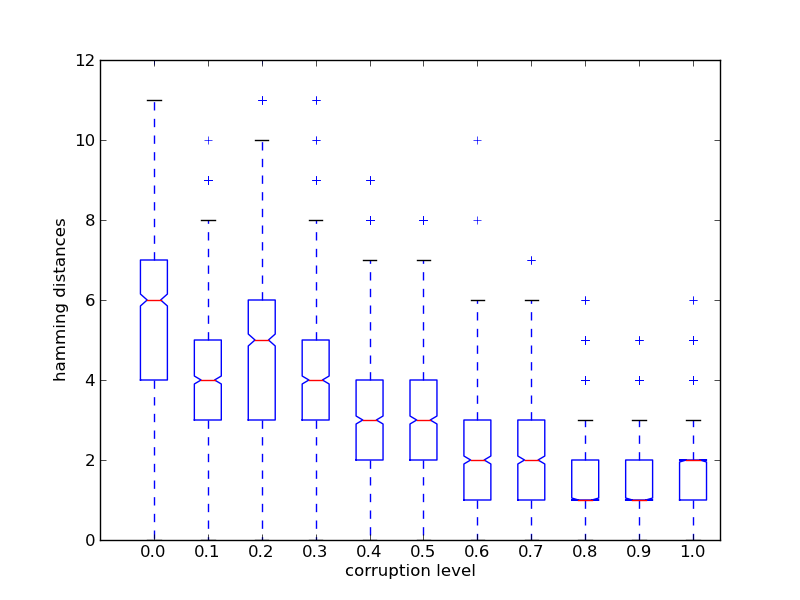
\includegraphics[width = 0.6\textwidth]{images/boxplots_basins.png}

\caption{Hamming distances to optimal solution on MaxOnes with different corruption levels.}
\label{figure:8bithiff}
\end{figure}

\begin{figure}[t!]
\center
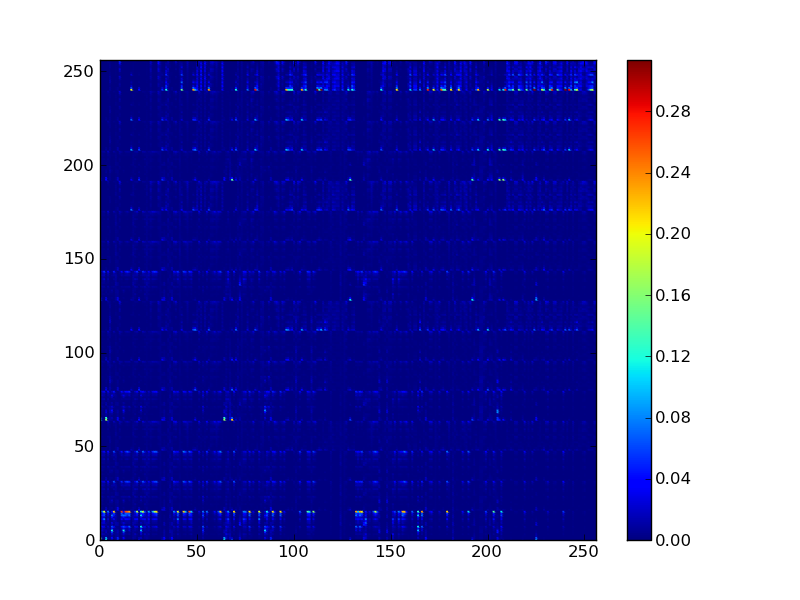
\includegraphics[width = 0.8\textwidth]{images/hiff-8-transition.png}

\caption{8-bit HIFF transition matrix.}
\label{figure:8bithiff}
\end{figure}

\subsection{Optimisation Algorithm}

The pipeline of the \emph{Denoising Autoencoder Genetic Algorithm} (DAGA) is similar to other EDAs and is inspired by methods in HBOA \cite{hboa}. A population of solutions is maintained, \(P_t\), and updated at each iteration, \(t\). An initial population of solutions, \(P_0\), is drawn from a uniform distribution. These solutions are evaluated and the fittest unique x\% are selected (i.e. truncation selection) to be in the training set, \(\hat{P_t}\). The Denoising Autoencoder, \(D_t\), is then trained with \(\hat{P_t}\) for \(e\) epochs. Following training, a new set of solutions, \(S_t\), is selected from \(P\) using tournament selection (with replacement). Each member of \(S_t\) is inputted to \(D_t\), and the output vector, \(y\), is sampled from using a binomial distribution, to produce a new solution. This solution is included in \(P_{t+1}\) if it is better than its closest neighbour according to Restricted Tournament Selection (RTR) \cite{hboa}. Pseudocode for DAGA is presented in Algorithm 1.

\section{Experiments}
\label{sec:experiments}
DAGA is tested on three sets of experiments: (1) discrete, (2) continuous and (3) accumulation of adaptation problems. 

\subsection{Discrete}
\subsubsection{Multi-dimensional Knapsack Problem}
Here we wish to choose of subset of \(N\) items to maximise the total value of items, \(z\), while satisfying \(m\) constraints. We wish to maximise:
\vspace{2mm}\\
\(z = \sum_{j=1}^{N} v_jx_j\), subject to \(\sum_{j=1}^{N} w_{ij}x_i \leq c_i, i = 1, ..., m\)
\vspace{2mm}\\
\(x_i \in \{0,1\}, j = 1, ..., N\).
\vspace{2mm}\\
Two different instances are used in the results presented below. The first is the Weing8 instance \cite{ref}, which has 105 items and two constraints (optimal solution is 602,319), and the second is a randomly generated instance with 500 items and one constraint (optimal solution is 100,104). Both instances are available in the supplementary material. If any of the \(m\) constraints are violated, the total value of chosen items is multiplied by \(-1\).

\subsubsection{Hierarchical If and only If}

The Hierarchical If and only If (HIFF) problem was created by Watson et al., as an example of a function which is not separable \cite{ref}. It is a pathological function for a hill climber because of a very large number of local optima. The HIFF is structured as a balanced binary tree \cite{hboa}, where at each lower level a transfer function is applied to consecutive non-overlapping 2-bit partitions, 00 \(\rightarrow\) 0, 11 \(\rightarrow\) 1, anything else \(\rightarrow\) null, to define the string in the layer above. At each level, 00 and 11 blocks contribute to the fitness by \(2^{level}\). Two global optima exist, a string of all 1s and all 0s. In the results section, DAGA is applied to the 128-bit HIFF. In order to remove any possible bias towards an all 1s solution, solutions from DAGA have a random bit mask (fixed before each trial) applied to them before evaluating fitness.

\subsubsection{Royal Road}
The Royal Road function as defined by Mitchell et al. \cite{mitchell}, divides a bit string, \(x\), into a number of  equally sized, non-overlapping partitions, \(z_i\in[x_i, ..., x_{i+n}])\). If all of the bits in the partition match a predefined pattern, \(s_i\) , then the partition's fitness contribution is added to the overall fitness. The existence of these ``Building blocks" was meant to act as a ``royal road" for GAs compared to hill-climbers but bad alleles hitchhiking to good partial solutions slows down convergence speed. The 128-bit problem with 8-bit partitions is defined as,
\\
\[
    f(x)= \sum_{i=1}^{16} \delta_i(x)o(s_i), \text{where } \delta_i(x)
\begin{cases}
    1,& \text{if } x\in s_i\\
    0,              & \text{otherwise}
\end{cases}
\] 
If a string contains two instances of s, a fitness of 16 is achieved. If all instances are found, fitness = 128. \(s_i\) instances are blocks of all 1s but as with the HIFF, a random mask is applied to the output of DAGA before fitness evaluation.
\subsubsection{MAXSAT}
\subsection{Continuous}
\subsubsection{Sphere}
\subsubsection{Rosenbrock}
\subsubsection{Rastrigin}
\subsection{Accumulation of Adaptation}
To answer the question of whether solving previous problems can speedup convergence on unseen problems in the same class, a new task was devised that was influenced by Watson et al \cite{watson_evolution}. DAGA is applied to solve three problems in sequence, without reinitialising the weights of the DA. The problems consist of minimising the hamming distance to a target string. The algorithm is evaluated on the difference in the number of iterations needed to solve the third problem after solving the first two, compared to solving the third problem on its own. The first and second solutions are a square and cross pattern. The third solution is a pattern made by recombining quarters from the original patterns. As each new solution can inherit a quarter from either the cross or the square pattern, there are \(2^4\) unique solutions. DAGA is tested on training on the cross and the square and then on one of the 16, as well as the square and the cross and then on of the other, leading to 32 experiments. 

\section{Results}
On the discrete and continuous problems, DAGA is compared to a canonical generational Genetic Algorithm (GA). On the continuous problems it is additionally compared to a (1+1)-ES with the 1/5 rule \cite{Igel benchmarking}. The GA employs tournament selection, two point crossover (with probability \(p_c\)) and on the discrete problems there is a probability, \(p_m\), of a bit flip mutation at each allele, while on the continuous problems there is probability, \(p_m\), of adding Gaussian noise to each component of the vector from \(N(0, \delta)\). Programming code is available in the online supplementary material.  For each experiment a large parameter sweep was performed on both DAGA and the GA and the best found configurations were chosen for comparison. Due to the stochastic nature of the algorithms each experiment is repeated 10 times.
\subsection{Discrete}
Table~\ref{table:main_results} presents details of the best solution in the population at quarter intervals of a run for DAGA and the GA on the 6 problems described above in 4.1. The table shows that DAGA finds either significantly better solutions, or optimal solutions significantly faster than the GA. On three of the five experiments (both knapsacks and MAXSAT), DAGA finds significantly better solutions than the GA, within the given evaluation limits. On the Weing8 knapsack instance DAGA reaches the optimum solution 8 out of 10 attempts, and on the 500-item instance 7 out of 10 attempts. On the MAXSAT instance, DAGA also reaches the optimum 70\% of the time. On all three of these problems the GA is unable to locate the optimal solution a single time. On the 128-bit HIFF, DAGA locates the optimal solution every time, while the GA locates it on only half of the trials. On the Royal Road, DAGA again locates the global optima on every trial, while the GA finds it on 9 out of 10. These results show that on a wide range of discrete problems DAGA is able to find higher quality solutions and more consistently locate the optimum compared to a GA.

 \begin{table}[t!]
    \begin{tabular}{ | p{1.8cm} | l | l | l | l | l | l | l | l | p{1cm} |}
    \hline
    Experiment & Algorithm & Min & Max & Mean 1Q & Mean 2Q & Mean 3Q & Mean 4Q & Success \%\\ \hline
    MAXSAT & GA & 424.0 & 429.0 & 425.9 & 426.2 & 426.3 & 426.5 & 0\%\\ 
    & AE & 429.0 & 430.0 & 429.1\(^*\) & 429.56\(^*\) & 429.67\(^*\) & 429.78\(^*\) & 70\%\\ \hline
    HIFF & GA & 832.0 & 1024.0 & 505.2 & 756.6 & 915.2 & 940.8 & 50\%\\   
    & AE & 1024.0 & 1024.0 & 568.4\(^*\) & 992.0\(^*\) & 1024.0\(^*\) & 1024.0 & 100\%\\   \hline
    Knapsack Weing8 & GA & 619568.0 & 621086.0 & 609728.9 & 619170.1 & 619856.0 & 620099.2 & 0\%   \\
    & AE & 621086.0 & 624319.0 & 617593.2\(^*\) & 621446.8\(^*\) & 622056.4\(^*\) & 623124.3\(^*\) & 80\% \\\hline
    Knapsack 500 & GA & 10047.0 & 10093.0 & 9637.7 & 10011.8 & 10055.8 & 10074.2 & 0\%   \\
    & AE & 10096.0 & 10104.0 & 10020.0\(^*\) & 10101.4\(^*\) & 10102.7\(^*\) & 10102.7\(^*\) & 70\% \\\hline
    RR & GA & 120.0 & 128.0 & 120.0 & 124.0 & 127.2 & 127.2 & 90\%   \\
    & AE & 128.0 & 128.0 & 122.4 & 128.0 & 128.0 & 128.0 & 100\% \\\hline
    \end{tabular}
    \label{table:main_results}
    \caption{Results for DAGA and the GA on the 5 problems. Showing the value of the minimum and maximum solution returned at the end of search, and the mean best solution in the population after 25\%, 50\%, 75\% and 100\% of evaluations had been completed, across 10 trials. Stars indicate that the mean result for DAGA is significantly different from the GA according to a Wilcoxan Rank Sum test (\(p<0.05\)).}
\end{table}

As well as frequently obtaining better quality solutions at the end of the optimisation process, DAGA also finds significantly better solutions than the GA at earlier stages in the optimisation process on a number of the tested problems. Table~\ref{table:main_results} shows the mean best solution found after different numbers of function evaluations have passed. From this we see that on all of the problems, apart from RR, DAGA finds significantly better solutions than the GA after a quarter of function evaluations have passed. On the 128-bit HIFF and RR functions, the GA is able to locate optimal solutions eventually but not consistently. DAGA is statistically significantly better after 25\%, 50\% and 75\% of evaluations have passed on the 128-bit HIFF. On this difficult problem, DAGA finds the optimum after 230,000 evaluations on average, with 200,000 in the fastest case and 285,000 in the slowest. At its fastest, the GA finds the optimum after 300,000 evaluations (mean 332,000 on the successful attempts), although on half the trials it fails to reach the optimum after 500,000. On RR, DAGA has a better mean score from the first quarter onwards, but the GA regularly reaches the optimum solution and their scores are not significantly different statistically (p=0.13 from 25\% to 50\%).

\subsection{Continuous}
Results for DAGA, (1+1)-ES and the GA are presented in for the sphere, Table~\ref{table:continuous_results} Rosenbrock and Rastrigin functions. On all three of these problems DAGA outperforms the GA, and is able to reach significantly better solutions with fewer evaluations. However, the (1+1)-ES is considerably better on the sphere and Rosenbrock functions, achieving significantly better solutions in the first quarter of evaluations (25,000 and 75,000 respectively) than DAGA can over the whole run (100,000 and 300,000). This implies that the (1+1)-ES is a much more efficient continuous optimiser on these search spaces. However, the (1+1)-ES performs extremely badly on the Rastrigin, which consists of many local optima. Here, the population-based GA and DAGA excel, getting much closer to the optimal solution of 0. DAGA is significantly better than the GA and the only algorithm to find solutions under 1.0. 
 \begin{table}[t!]
    \begin{tabular}{ | p{1.8cm} | l | l | l | l | l | l | l | l | |}
    \hline
    Experiment & Algorithm & Min & Max & Mean 1Q & Mean 2Q & Mean 3Q & Mean 4Q \\ \hline
    Sphere 50D & GA & 0.065 & 0.101 & 25.178 \(\pm\)10.900 & 0.165 \(\pm\)0.088 & 0.125 \(\pm\)0.032 & 0.088 \(\pm\)0.016\\
    & (1+1)-ES & 0.000 & 0.000 & 0.000 \(\pm\)0.000 & 0.000 \(\pm\)0.000 & 0.000 \(\pm\)0.000 & 0.000 \(\pm\)0.000\\
    & AE & 0.026 & 0.033 & 0.376 \(\pm\)0.016 & 0.055 \(\pm\)0.004 & 0.037 \(\pm\)0.002 & 0.029 \(\pm\)0.003\\\hline
    Rosenbrock 10D & GA & 0.547 & 0.800 & 5.092 \(\pm\)1.371 & 2.026 \(\pm\)0.930 & 0.830 \(\pm\)0.133 & 0.659 \(\pm\)0.106\\
    & (1+1)-ES & 0.000 & 0.000 & 0.003 \(\pm\)0.000 & 0.000 \(\pm\)0.000 & 0.000 \(\pm\)0.000 & 0.000 \(\pm\)0.000\\
    & AE & 0.018 & 0.082 & 0.117 \(\pm\)0.033 & 0.058 \(\pm\)0.022 & 0.049 \(\pm\)0.019 & 0.042 \(\pm\)0.018\\\hline
     Rastrigin 10D & GA & 1.395 & 4.347 & 3.132 \(\pm\)1.245 & 3.098 \(\pm\)1.232 & 3.047 \(\pm\)1.284 & 3.058 \(\pm\)1.234\\ 
    & (1+1)-ES & 37.808 & 160.187 & 89.844 \(\pm\)33.520 & 89.844 \(\pm\)33.520 & 89.844 \(\pm\)33.520 & 89.844 \(\pm\)33.520\\
    & AE & 0.601 & 1.277 & 1.145 \(\pm\)0.327 & 1.002 \(\pm\)0.275 & 0.945 \(\pm\)0.209 & 0.888 \(\pm\)0.203\\\hline
    \end{tabular}
    \label{table:continuous_results}
    \caption{Results for DAGA, (1+1)-ES and the GA on 3 continuous problems. Showing the value of the minimum and maximum solution returned at the end of search, and the mean best solution in the population after 25\%, 50\%, 75\% and 100\% of evaluations had been completed, across 10 trials. A 100,000 evaluation limit is used on sphere and 300,000 is used on the other two.  On each function results were found to have significant differences on a one way ANOVA (\(p<0.05\)), post-hoc analysis with a t-test and the Bonferroni correction for multiple comparisons showed significant differences between all pairs (\(p<0.05\)).}
\end{table}


\subsection{Accumulation of Adaptations}
Results for DAGA on the image generation task described in Section 4.3 are presented in Table x. The figure shows the difference in the average number of iterations taken to solve the third problem, between solving the third problem directly and solving it after using a dA that has been trained on solving the first two problems without reinitialisation. We see that in every case, there is a significant speed up when DAGA solves the first two problems before solving the third. Figure~\ref{figure:experiment_subplots}(a) shows the population created by sampling random inputs after solving the Cross and Box problems, while Figure~\ref{figure:experiment_subplots}(b) shows the same without training. There is a clear difference in the solutions created, with the dA after training showing box-like pattern, mixed with diagonals. This shows that it has learnt from both training patterns, and the large speed ups on the third task shows that is exploited to solve the latter problem considerably faster. Unsurprisingly, the largest speed ups occur when the third problem is identical to the second. For both initial training patterns, this speedup is considerably greater than the mean, although it is markedly greater on the Box-Cross (BC) set. Also notable on BC is that the speed up is much less on the Box pattern, even though it was solved in the first run of the algorithm. By training on the Cross pattern second, we may lose a lot of the information learnt from the first run. On BC, apart from the Cross, the most speed up is seen in solutions which inherit \(1/4\) from the Box and \(3/4\) from the Cross. The reverse is not true, and for CB there are large savings on the Cross, which it was trained on initially as well as the \(1/4\)Box, \(3/4\)Cross solution that BC performs well on. Figure~\ref{figure:experiment_subplots} (b) and (c) shows that while BC and CB both share features of the two root patterns, they are dominated by the second trained pattern. The Cross patterns are more sparse, which could explain why it takes longer to produce a Box. In order to reduce the memory effect, it may help to use a lower learning rate. However, this simple example illustrates that dAGA is able to transfer learned structure between tasks.

 \begin{table}[t!]
    \begin{tabular}{ | l | l | l | l | l | l | l | l | l | l | l | l | l| l| l| l|}
    \hline
    & a &b &c &d &e &f &g &h &i &j &k &l &m &n &p \\ \hline
    a then p & 21.91 & 33.64 & 18.82 & 46.09 & 10.00 & 27.82 & 11.09 & 84.09 & 46.27 & 42.18 & 43.55 & 63.45 & 44.18 & 53.45 & 173.64\\\hline
    p then a & 117.36 & 63.18 & 46.55 & 65.91 & 54.45 & 62.36 & 44.18 & 91.55 & 74.82 & 61.27 & 55.91 & 57.00 & 72.18 & 70.36 & 125.18\\\hline
    \end{tabular}
    \label{table:accumulation_results}
    \caption{Showing the difference between mean number of iterations taken to solve the image labelled on the top row without pre-learning and the mean number of iterations taken with pre learning on the two solutions labelled in the first column, averaged over 10 trials. All mean iterations are significantly different, Wilcoxan Rank Sum test (\(p<0.05\)). NOTE: MISSING O!!!!}
\end{table}

\begin{figure}[t!]
\center
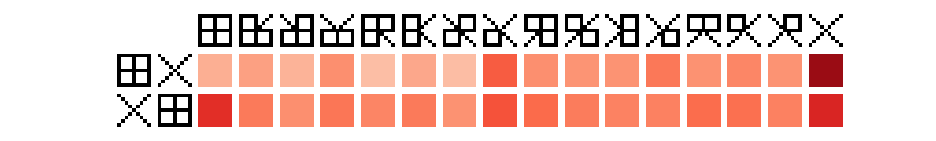
\includegraphics[width = 1.0\textwidth]{images/boxy_square_cmap.png}

\caption{Showing the difference between mean number of iterations taken to solve the image pictured on the top row without pre-learning and the mean number of iterations taken with pre learning on the two solutions pictured in the first column, averaged over 10 trials.} 
\label{figure:cross_square_grid}
\end{figure}

\begin{figure}[!]
\centering
\subfigure[]{
\makebox[.5\textwidth]{
    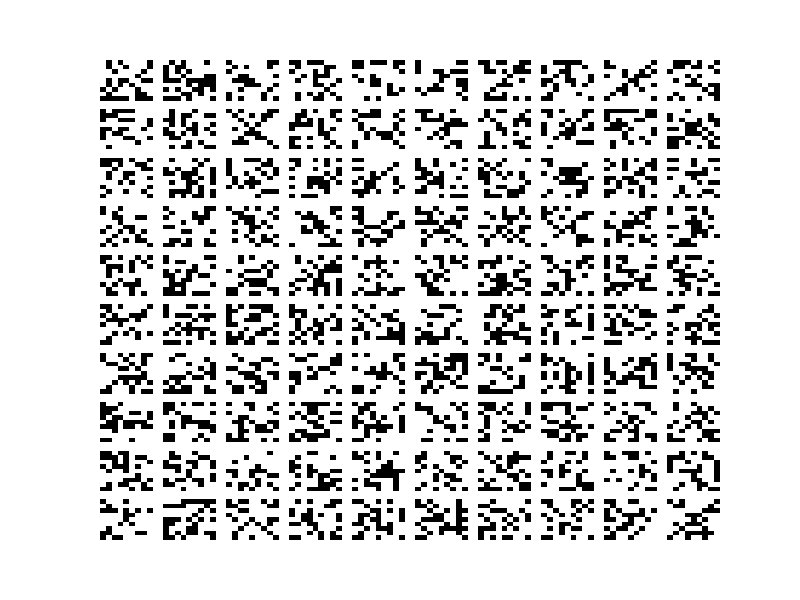
\includegraphics[scale=0.5]{images/lots_of_crossies.png}
    \label{fig:subfig1}
    %\caption{After solving the box and cross}
    }
}
\subfigure[]{
\makebox[.5\textwidth]{
    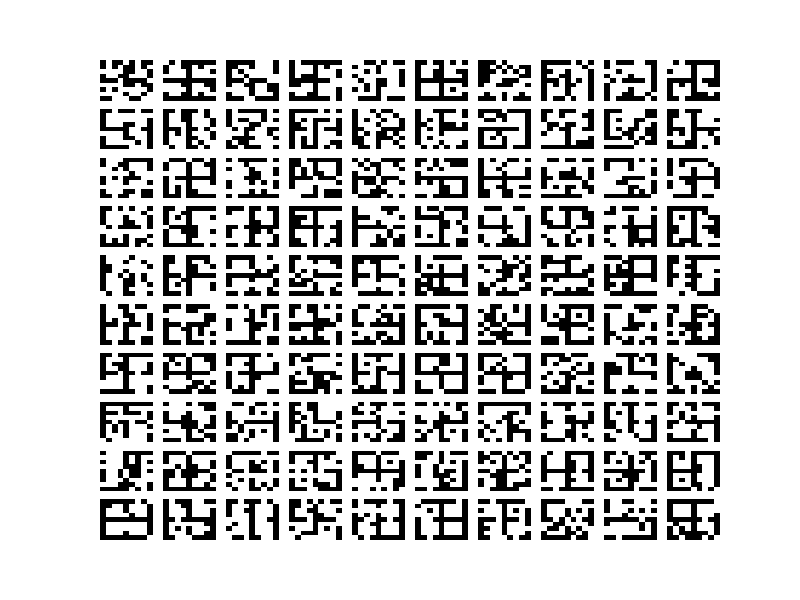
\includegraphics[scale=0.5]{images/first_pop.png}
    \label{fig:subfig1}
    %\caption{After solving the box and cross}
    }
}
\subfigure[]{
\makebox[.5\textwidth]{
    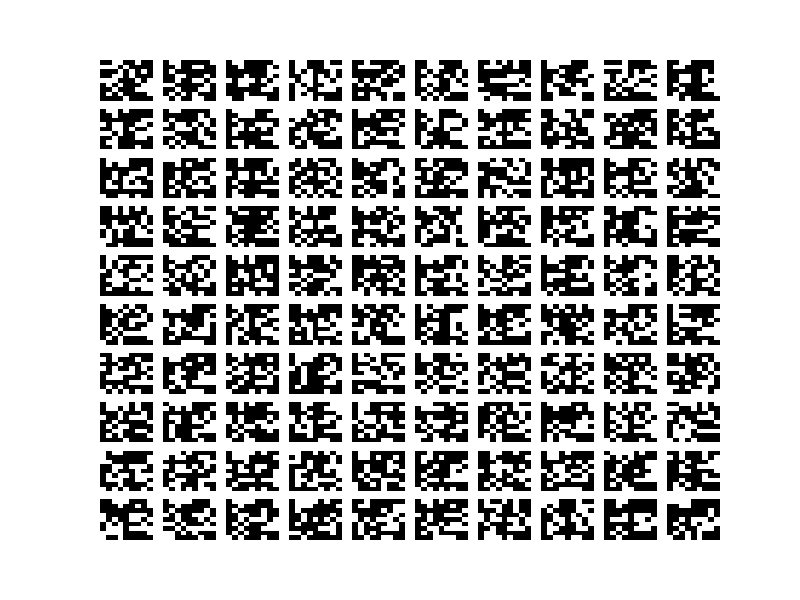
\includegraphics[scale=0.5]{images/no_learning.png}
    \label{fig:subfig2}
    %\caption{Start of training}
    }
}
\caption[Optional caption for list of figures]{Showing the output of 100 random inputs passed through the autoencoder (a) after solving the cross and then the box tasks and (b) at the start of the optimisation process.}
\label{figure:experiment_subplots}
\end{figure}
\section{Discussion}
% HyperPothesis: When the input features are independent then high corruption helps because you don't care about information in the input as much, and you're forcing solutions to have a similar structure (the output structure is not dependant on the input structure because independent. On structured problems like the HIFF there is a lot of information in the inputs, so distorting this discards the information that might be useful.)

\section{Conclusion}

\subsubsection*{Acknowledgments.} The work is funded by the FQEB Templeton grant ``Bayes and Darwin", and the FP-7 FET OPEN Grant INSIGHT.

\bibliographystyle{splncs}
\bibliography{autoencoder_ppsn}

\end{document}
